\section{Graph}
The graph is generated when the game/map is loaded. We’ve decided that our graph is a grid-like graph. We start off with generating the nodes, after that we generate adjacency edges. A node can have a maximum of 8 edges. When a static object is placed we remove edges from the node(s) on which the object is placed upon. We also remove the edges that lead to the node(s) on which the object is placed.

There is a GraphManager which is a Singleton class to avoid making multiple graphs. It's also easy to access the graph in different parts of the code due to the GraphManager. 

\begin{figure}[!htb]
    \centering
    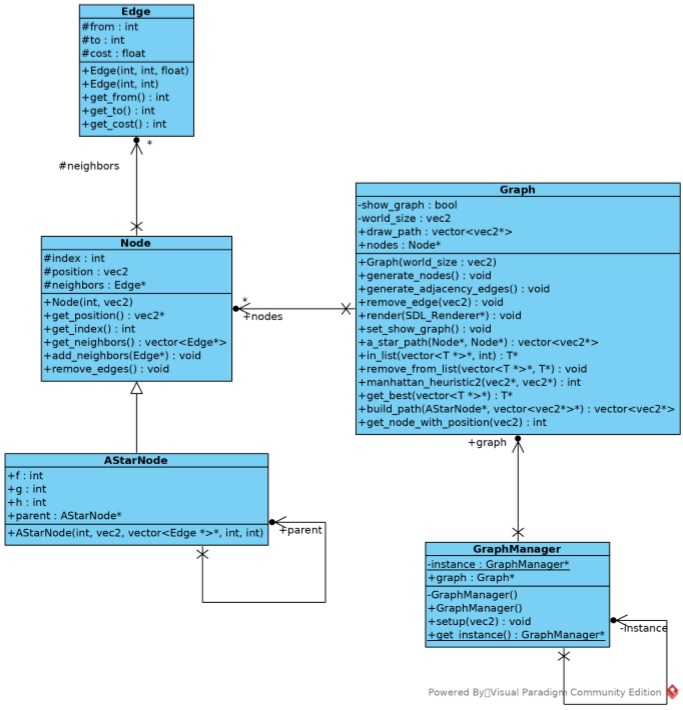
\includegraphics[scale=0.75]{res/graph.jpg}
    \caption{Class diagram for the Graph.}\label{fig:blue-line}
\end{figure}